\section{Definizioni e propriet\`a di base}\label{sec:definizioni-e-proprieta-di-base}

In questa sezione saranno proposte definizioni e propriet\`a di base di una struttura dati per la rappresentazione
di gerarchie di grafi a pi\`u livelli, in cui sia possibile ottenere informazioni sull'intera struttura gerarchica in
relazione ai singoli grafi che la compongono, come attraverso l'espansione e la contrazione di nodi.
In particolare, riprendendo dalla terminologia e dai concetti esistenti in letteratura, si proporranno definizioni
originali di \textit{grafo decontraibile} e di \textit{grafo multi-livello}.

\subsection{Grafo decontraibile}

A partire dal concetto noto di grafo quoziente e di contrazione, si vuole definire una particolare
tipologia di grafi quoziente che, oltre a rappresentare le caratteristiche strutturali ad alto livello di astrazione
dei grafi da cui sono derivati, siano in grado di mantenere l'informazione originale di questi ultimi, in
che modo essa sia legata alla sua rappresentazione astratta. \newline
Nasce così il concetto di grafo decontraibile, che intuitivamente pu\`o essere considerato come un grafo
in cui i nodi sono riconducibili ad un grafo e gli archi ad un insieme di archi tra i nodi dei grafi
associati ai nodi coinvolti.
\newpage

\begin{definition}[Grafo Decontraibile]
    Un \textbf{grafo decontraibile} \`e una quadrupla $G = (V, E, dec_V, dec_E)$ dove:
    \begin{itemize}
        \item $V$ \`e un insieme di elementi detti \textbf{supernodi};
        \item $E \subseteq V \times V$ \`e un insieme di coppie ordinate di supernodi, dette \textbf{superarchi};
        \item $dec_V : V \rightarrow \mathcal{G}_D$ \`e una funzione tale per cui $dec_V(v) = (\mathcal{V}_v,
            \mathcal{E}_v, dec_{\mathcal{V}_v}, dec_{\mathcal{E}_v})$ \`e un grafo decontraibile rappresentato
            dal supernodo $v$;
        \item $dec_E : E \rightarrow (\mathcal{V} \times \mathcal{V})$ con $\mathcal{V} = \bigcup_{v \in V}\mathcal{V}_v$,
            \`e una funzione tale per cui $\forall$ $ e = (u, v)$, $dec_E(e) = \mathcal{E}_e \subseteq$ $\{(a, b)$ $\mid$ $a \in \mathcal{V}_u$ $\wedge$
            $b \in \mathcal{V}_v\}$ \`e un insieme di archi rappresentati dal superarco $e$.
    \end{itemize}
\end{definition}

Nella definizione, cos\`{i} come d'ora in avanti, si utilizzer\`a la notazione $\mathcal{G}_D$ per indicare l'insieme
dei grafi decontraibili, e le notazioni $\mathcal{V}$ e $\mathcal{E}$ per
indicare, rispettivamente, insiemi di supernodi e superarchi ottenibili attraverso decontrazioni e, quindi, di
livello inferiore rispetto al grafo decontratto di riferimento.
Le notazioni $\mathcal{V}_v$ e $\mathcal{E}_v$ saranno utilizzate per indicare, rispettivamente,
insiemi di nodi e archi di grafi ottenibili attraverso la decontrazione di un certo supernodo $v$.
Nel contesto di un determinato grafo decontraibile, per portare maggiore distinzione si continuer\`a ad utilizzare
il termine di nodo ed arco per riferirsi ai supernodi e superarchi di tale livello inferiore. \newline

Si noti che \`e possibile usare una notazione basata su attributi, alternativa a quella delle funzioni, per
descrivere le propriet\`a caratteristiche di nodi ed archi che rendono tale un grafo decontraibile.
Tale notazione sar\`a utilizzata in seguito per semplificare la descrizione di algoritmi. \newline
In particolare, si pu\`o definire un grafo decontraibile come un normale grafo diretto sotto forma di coppia
$(V, E)$ dove:
\begin{itemize}
    \item $\forall$ $v \in V,$ \`e definito un attributo $v.dec = G_v$ dove $G_v = (\mathcal{V}_v, \mathcal{E}_v)$ \`e un
        grafo decontraibile rappresentato da $v$, quindi tale per cui $dec_V(v) = v.dec$.
    \item $\forall$ $e=(u, v)$  $\in E$, \`e definito una attributo $e.dec = E_e$ dove \\
        ${\mathcal{E}_e \subseteq \{(a, b) \mid a \in \mathcal{V}_u \wedge b \in \mathcal{V}_v\}}$ \`e un insieme di archi
        rappresentati da $e$, quindi tale per cui $dec_E(e) = e.dec$.
\end{itemize}

Si consideri la natura ricorsiva definizione di grafo decontraibile, per cui se un supernodo $v$ pu\`o essere
rappresentato da un grafo decontraibile $G_v$, allora i nodi di $G_v$ saranno a loro volta dei supernodi.
Stessa cosa vale per gli archi, che possono essere rappresentati da insiemi di archi tra i nodi dei grafi.
La scelta di rendere il grafo decontraibile una struttura ricorsiva, cos\`{i} come la definizione in sé stessa,
\`e utile alle successive definizioni legate ai grafi multi-livello. \newline

\begin{figure}[h!]
\centering
\begin{tikzpicture}
  [mynode/.style={draw, thick, circle, size=0.3mm},
    myarrow/.style={thick, -Triangle},
    ->,shorten >=1pt,auto,node distance=2cm, thick,main node/.style={circle,draw}]

  % Nodes
  \node[main node] (A) {v$_1$};
  \node[main node, blue] (B) [right of=A] {v$_2$};
  \node[main node, blue] (C) [below right of=B] {v$_3$};
  \node[main node] (D) [below left of=C] {v$_4$};

  % Edges
  \path[every node/.style={font=\sffamily\small}];
  \draw[myarrow](A) to node [above] {$e_1$} (B);
  \draw[myarrow, blue] (B) to node [above, name=e2] {$e_2$} (C);
  \draw[myarrow](C) to node [above] {$e_3$} (D);
  \draw[myarrow](B) to node [left] {$e_4$} (D);

  % G_b graph
  \begin{scope}[shift={(6,1)}]
  \draw[blue] (0,0) circle (1.5cm);
  \node[main node] (X) at (-0.5,0.5) {a$_1$};
  \node[main node] (Y) at (1,0) {a$_2$};
  \node[main node] (Z) at (0,-1) {a$_3$};
  \draw[myarrow] (X) -- (Y);
  \draw[myarrow] (Y) -- (Z);
  \draw[myarrow] (Z) -- (X);
  \end{scope}

  % G_c graph
  \begin{scope}[shift={(8,-2.5)}]
  \draw[blue] (0,0) circle (1.5cm);
  \node[main node] (T) at (-0.5,0.5) {a$_4$};
  \node[main node] (U) at (1,0) {a$_5$};
  \node[main node] (V) at (0.25,-1) {a$_6$};
  \node[main node] (W) at (-0.5,-0.5) {a$_7$};
  \draw[myarrow] (U) -- (T);
  \draw[myarrow] (U) -- (W);
  \draw[myarrow] (U) -- (V);
  \end{scope}

  % edges between graphs
  \draw[myarrow, blue] (Z) -- (T);
  \draw[myarrow, blue] (Y) -- (U);

  % Links
  \draw[dashed, line width=1.5pt, red] (B) to[out=65, in=145] node {$dec_{V}(v_2)$} (4.5,1);
  \draw[dashed, line width=1.5pt, red] (e2) to[out=0, in=155] node [below] {$dec_{E}(e_2)$} (6.75,-1);
  \draw[dashed, line width=1.5pt, red] (e2) to[out=0, in=175] (8,-0.7);
  \draw[dashed, line width=1.5pt, red] (C) to[out=300, in=145] node [below] {$dec_{V}(v_3)$} (6.5,-2);
\end{tikzpicture}
\vspace{-15pt}
\caption{Un esempio di decontrazione locale di un grafo decontraibile}
\label{fig:dec-graph-example}
\end{figure}

In Figura~\ref{fig:dec-graph-example} \`e mostrato un esempio di grafo decontraibile sulla sinistra, mentre sulla
destra sono rappresentati i grafi associati ai supernodi $v_2$ e $v_3$, assieme all'insieme di archi associato
al superarco $e_2$.
Si osservi che il grafo $dec_V(v_2)$ composto dai nodi $a_1$, $a_2$ e $a_3$, ad esempio, manca degli archi collegati
esternamente che definiscono il contesto in cui tale grafo si colloca, e solo uno degli archi incidenti
in $v_1$ \`e stato espanso.
Questo fornisce una visione parziale dell'informazione contenuta nel grafo decontraibile a sinistra,
e per questo si pu\`o dire che il grafo a destra \`e il risultato di un'espansione locale. \newline

Inoltre, dal momento in cui i grafi decontraibili sono a tutti gli effetti dei grafi, tutte le
definizioni date sui grafi standard continuano ad essere utilizzate in modo equivalente per i grafi decontraibili.
Analogamente, un supernodo pu\`o essere considerato come un particolare tipo di nodo, e lo stesso vale per i
superarchi.
In particolare, il concetto di isomorfismo pu\`o essere esteso ai grafi decontraibili senza particolari modifiche,
ignorando l'aspetto ``decontraibile'' di nodi e archi, ovvero ignorando le funzioni $dec_V$ e $dec_E$ di entrambi
i grafi di cui si vuole valutare l'isomorfismo.

% Potrebbe essere altres\`{i} utile indicare un tipo di isomorfismo specifico per i grafi decontraibili, che tenga
% conto delle funzioni di decontrazione, ovvero che imponga un isomorfismo anche tra i grafi risultanti dalle
% decontrazioni dei singoli nodi, risultando in una forma di isomorfismo pi\`u forte.

% \begin{defintion}[Isomorfismo forte di Grafi Decontraibili] \newline
%    Siano $G = (V, E)$ e $H = (W, F)$ due grafi decontraibili, essi si dicono \textbf{fortemente isomorfi} se
%     esiste una biiezione $f : V \rightarrow W$ tale per cui
%     \begin{itemize}
%        \item $(u, v) \in E$ se e solo se $(f(u), f(v)) \in F$ per ogni $u, v \in V$
%        \item $dec_V(u)$ \`e fortemente isomorfo a $dec_V(f(u))$ per ogni $u \in V$
%        \item
%    \end{itemize}

%\end{defintion}

\nlparagraph{Contrazioni di grafi decontraibili}\label{subsec:contrazioni}

A partire dalla decontrazione, che rappresenta un aspetto intrinseco alla definizione dei grafi decontraibili,
la relazione di contrazione \`e quella che, intuitivamente, permette di legare grafi decontraibili nel senso
opposto.
Se da un lato la decontrazione permette di costruire grafi che rappresentino espansioni locali, con una
definizione di contrazione si vogliono stabilire le condizioni che permettono di legare interi grafi decontraibili
ad altri che ne forniscano una loro rappresentazione astratta, affinch\`e la tale rappresentazione
sia coerente con il concetto di contrazione esistente nella teoria dei grafi.

\begin{definition}[Contrazione di un Grafo Decontraibile]
    Sia $G = (V, E, dec_V, dec_E)$ un grafo decontraibile, il grafo decontraibile \\
    $G\mathcal{'} = (\mathfrak{V}, \mathfrak{E}, dec_{\mathfrak{V}}, dec_{\mathfrak{E}})$ \`e una sua
    \textbf{contrazione} se e solamente se:
        \begin{itemize}
            \item l'insieme $\{V_\alpha \mid \alpha \in \mathfrak{V}\}$ \`e una partizione di $V$
            \item l'insieme $(\{E_\alpha \mid \alpha \in \mathfrak{V}\} \setminus \{ \emptyset \}) \cup
                \{ dec_{\mathfrak{E}}(\epsilon) \mid \epsilon \in \mathfrak{E}\}$ \`e una partizione di $E$.
        \end{itemize}
\end{definition}

Nella definizione, cos\`{i} come d'ora in avanti, si utilizzer\`a la notazione $\mathfrak{V}$ e $\mathfrak{E}$ per
indicare, rispettivamente, gli insiemi di supernodi e superarchi di un grafo contratto, e quindi di livello
superiore rispetto al grafo di riferimento.

Nella Figura~\ref{fig:contraction-example}, sulla sinistra \`e mostrato un esempio di grafo decontraibile
contrazione del grafo decontraibile a destra, dove sono annotati per ogni supernodo e superarco
i nodi e gli archi ottenibili dalle loro decontrazioni. \newline

\begin{figure}
    \centering
    \begin{tikzpicture}
    [mynode/.style={draw, thick, circle, size=0.3mm},
    ->,shorten >=1pt,auto,node distance=2cm, thick, main node/.style={circle,draw}]

        % Nodes
        \node[main node,
          label={[align=center, blue, font=\tiny]above:{$V_{v_1} = \{a_1, a_2\}$}\\{$E_a = \emptyset$}}]
        (A) {$v_1$};
        \node[main node,
        label={[align=center, blue, font=\tiny]above:{$V_{v_2} = \{a_3, a_4, a_5\}$}\\{$E_{v_2} = \{(a_3, a_4),$}\\{$(a_4, a_5), (a_5, a_3)\}$}}]
        (B) [right of=A, node distance=2.5cm] {$v_2$};
        \node[main node,
        label={[align=left, blue, font=\tiny]right:{$V_{v_3} = \{a_6, a_7, a_8, a_9\}$}\\{$E_{v_3} = \{(a_7, a_6),$}\\{$(a_7, a_9),(a_7, a_8)\}$}}]
          (C) [below right of=B] {$v_3$};
        \node[main node,
        label={[align=center, blue, font=\tiny]left:{$V_{v_4} = \{a_{10}\}$}\\{$E_{v_4} = \emptyset$}}]
          (D) [below left of=C] {$v_4$};

        % Edges
        \path[every node/.style={font=\sffamily\small}];
        \draw[myarrow](A) to node [above,
        label={[align=center, blue, font=\tiny]below:{$E_{e_1} = $}\\{$\{(a_2, a_5)\}$}}] {$e_1$} (B);
        \draw[myarrow](B) to node [above,
        label={[align=left, blue, font=\tiny]right:{$E_{e_2} = \{(a_5,a_6),$}\\{$(a_4, a_7)\}$}}] {$e_2$} (C);
        \draw[myarrow](C) to node [below,
        label={[align=left, blue, font=\tiny]right:{$E_{e_3} =$}\\{$ \{(a_9,a_{10}),$}\\{$ (a_8, a_{10})\}$}}] {$e_3$} (D);
        \draw[myarrow](B) to node [right, label={[align=right, blue, font=\tiny]left:{$E_{e_4} = \{(a_5,a_{10})\}$}}] {$e_4$} (D);

        % G_b graph
        \begin{scope}[shift={(9.5,1)}];
        \draw[blue] (0,0) circle (1.5cm);
        \node[above, blue] at (0,1.5) {$v_2$};
        \node[main node] (X) at (-0.5,0.5) {$a_3$};
        \node[main node] (Y) at (1,0) {$a_4$};
        \node[main node] (Z) at (0,-1) {$a_5$};
        \draw[myarrow] (X) -- (Y);
        \draw[myarrow] (Y) -- (Z);
        \draw[myarrow] (Z) -- (X);
        \end{scope}

        % G_c graph
        \begin{scope}[shift={(11.5,-1.75)}]
        \draw[blue] (0,0) circle (1.5cm);
        \node[right, blue] at (1.5,0) {$v_3$};
        \node[main node] (T) at (-0.5,0.5) {$a_6$};
        \node[main node] (U) at (1,0) {$a_7$};
        \node[main node] (V) at (0.25,-1) {$a_8$};
        \node[main node] (W) at (-0.5,-0.5) {$a_9$};
        \draw[myarrow] (U) -- (T);
        \draw[myarrow] (U) -- (W);
        \draw[myarrow] (U) -- (V);
        \end{scope}

        % G_a graph
        \begin{scope}[shift={(6.7, 1)}]
        \draw[blue] (0,0) circle (1cm);
        \node[above, blue] at (0,1) {$v_1$};
        \node[main node] (N) at (0,0.5) {$a_1$};
        \node[main node] (M) at (0,-0.5) {$a_2$};
        \end{scope}

        % G_d graph
        \begin{scope}[shift={(8.5,-2.5)}]
        \draw[blue] (0,0) circle (0.75cm);
        \node[left, blue] at (-0.75,0) {$v_4$};
        \node[main node] (K) at (0,0) {$a_{10}$};
        \end{scope}

        % edges between graphs
        \draw[myarrow, blue] (M) -- (Z);
        \draw[myarrow, blue] (Z) -- (K);
        \draw[myarrow, blue] (Z) -- (T);
        \draw[myarrow, blue] (Y) -- (U);
        \draw[myarrow, blue] (W) -- (K);
        \draw[myarrow, blue] (V) -- (K);
\end{tikzpicture}
    \caption{Esempio di contrazione di un grafo decontraibile}
    \label{fig:contraction-example}
\end{figure}

Dalla definizione si evince che le seguenti sono condizioni necessarie affinch\`e un grafo decontraibile $G'$ possa
essere una contrazione di un grafo decontraibile $G$:
\begin{enumerate}[(i)]
    \item I nodi di $G'$ devono avere tutti un grafo non vuoto come decontrazione, ovvero $V_\alpha \neq \emptyset$
    per ogni $\alpha \in \mathfrak{V}$.
    Infatti se fosse che $V_\alpha = \emptyset$ per qualche $\alpha \in \mathfrak{V}$, allora l'insieme
    $\{V_\alpha \mid \alpha \in \mathfrak{V}\}$ non costituirebbe una partizione di $V$, in quanto, per definizione,
    l'insieme vuoto non pu\`o essere incluso in una partizione.
    \item Gli insiemi di nodi delle decontrazioni dei supernodi in $G'$ devono essere a due a due disgiunti, ovvero
    non possono esistere nodi a cui corrispondono contemporaneamente due supernodi distinti, in quanto, anche in
    questo caso, l'insieme $\{V_\alpha \mid \alpha \in \mathfrak{V}\}$ non costituirebbe una partizione di $V$.
    \item I superarchi di $G'$ devono avere tutti una decontrazione non vuota.
    Infatti, se fosse che $dec_{\mathfrak{E}}(\epsilon) = \emptyset$ per qualche $\epsilon \in \mathfrak{E}$, allora
    l' insieme $(\{E_\alpha \mid \alpha \in \mathfrak{V}\} \setminus \{ \emptyset \}) \cup
    \{ dec_{\mathfrak{E}}(\epsilon) \mid \epsilon \in \mathfrak{E}\}$ non costituirebbe una partizione di $E$,
    analogamente a quanto detto nel punto (i). \newline
    Si noti che la condizione di disgiunzione tra gli insiemi di archi delle decontrazioni dei superarchi \`e
    automaticamente soddisfatta dalla definizione di grafo decontraibile e delle decontrazioni dei suoi archi.
\end{enumerate}

E' rilevante notare che, data una contrazione $G'$ del grafo decontraibile $G$, essa contiene tutte le informazioni
necessarie a calcolare la struttura di archi e nodi di $G$.
Infatti, sia $G' = (\mathfrak{V}, \mathfrak{E})$ una contrazione di $G$, allora dalla definizione si ha:

\begin{equation*}
    G = (\bigcup_{\alpha \in \mathfrak{V}} V_\alpha , \;
        (\bigcup_{\alpha \in \mathfrak{V}} E_\alpha \cup \bigcup_{\epsilon \in \mathfrak{E}}{dec_{\mathfrak{E}}(\epsilon)}), \;
        dev_V, \; dec_E) %TODO: \bigsqcup{\alpha \in \mathfrak{V}} dec_{V_{\alpha}}, (\bigsqcup{\alpha \in \mathfrak{V}} dec_{E_{\alpha}} \cup ???)
\end{equation*}

dove $dec_V$ è ottenuto dall'unione delle funzioni $dec_{\mathfrak{V}_v}$ per ciascun $v \in \mathfrak{V}$,
e $dec_E$ è ottenuto dall'unione delle funzioni $dec_{\mathfrak{E}_e}$ per ciascun $e \in \mathfrak{E}$ combinato con
tutte le mappature tra i superarchi in $\bigcup{\epsilon \in \mathfrak{E}} dec_{\mathfrak{E}}(\epsilon)$ e le loro
decontrazioni. \newline

Definiamo, quindi, l'operatore unario $.^D : \mathcal{G}_D \rightarrow \mathcal{G}_D$ come l'operatore di
\textbf{decontrazione completa} che, dato un grafo decontraibile $G = (V, E, dec_V, dec_E)$ restituisce il grafo
decontraibile $G^D$ ottenuto dalla decontrazione di tutti i supernodi e superarchi del grafo in input.

\begin{equation*}
    G^D = (\bigcup_{v \in V} \mathcal{V}_v , \; (\bigcup_{v \in V} \mathcal{E}_v \cup \bigcup_{e \in E} dec_E(e)), \;
    dec_{\mathcal{V}}, \; dec_{\mathcal{E}})
\end{equation*}

Una contrazione di un grafo decontraibile $G$ pu\`o, quindi, essere alternativamente definita come un suo grafo
quoziente decontraibile $G'$ la cui decontrazione completa $(G')^D$ \`e proprio $G$.
\newline

Si noti che, in generale, un grafo decontraibile $G$ pu\`o non essere una contrazione di $G^D$.
Questo pu\`o verificarsi unicamente quando $G$ non soddisfa tutte le condizioni (i), (ii) e (iii) presentate in
precedenza. \newline
Per rendere chiaro questo aspetto, in Figura~\ref{fig:non-contraction-example} \`e proposta una variazione
dell'esempio precedente, in cui il grafo decontraibile a sinistra, ottenuto come decontrazione completa del grafo
destra, non \`e una sua contrazione, in quanto il super-nodo $a_3$ appartiene contemporaneamente a $V_a$ e $V_b$,
violando la condizione (ii), e il super-arco $e_3$ viene decontratto in un insieme vuoto di archi,
violando la condizione (iii).

\begin{figure}
    \centering
    \begin{tikzpicture} [mynode/.style={draw, thick, circle, minimum size=0.3cm},
    ->,>={stealth},shorten >=1pt,auto,node distance=2cm,
    thick,main node/.style={circle,draw}]

    % Nodes
    \node[main node,
        label={[align=center, blue, font=\tiny]above:{$V_{v_1} = \{a_1, a_2, a_3\}$}\\{$E_a = \emptyset$}}]
    (A) {v$_1$};
    \node[main node,
        label={[align=center, blue, font=\tiny]above:{$V_{v_2} = \{a_3, a_4, a_5\}$}\\{$E_{v_2} = \{(a_3, a_4),$}\\{$(a_4, a_5), (a_5, a_3)\}$}}]
    (B) [right of=A, node distance=2.5cm] {v$_2$};
    \node[main node,
        label={[align=left, blue, font=\tiny]right:{$V_{v_3} = \{a_6, a_7, a_8, a_9\}$}\\{$E_{v_3} = \{(a_7, a_6),(a_7, a_9),$}\\{$(a_7, a_8)\}$}}]
    (C) [below right of=B] {v$_3$};
    \node[main node,
        label={[align=center, blue, font=\tiny]left:{$V_{v_4} = \{a_{10}\}$}\\{$E_{v_4} = \emptyset$}}]
    (D) [below left of=C] {v$_4$};

    % Edges
    \path[every node/.style={font=\sffamily\small}];
    \draw[myarrow](A) to node [above,
    label={[align=center, blue, font=\tiny]below:{$E_{e_1} = $}\\{$\{(a_2, a_5)\}$}}] {$e_1$} (B);
    \draw[myarrow](B) to node [above,
    label={[align=left, blue, font=\tiny]right:{$E_{e_2} = \{(a_5,a_6), (a_4, a_7)\}$}}] {$e_2$} (C);
    \draw[myarrow](C) to node [below,
    label={[align=left, blue, font=\tiny]right:{$E_{e_3} = \emptyset$}}] {$e_3$} (D);
    \draw[myarrow](B) to node [right, label={[align=right, blue, font=\tiny]left:{$E_{e_4} = \{(a_5,a_{10})\}$}}] {$e_4$} (D);

    % G_b graph
    \begin{scope}[shift={(8.5,1)}]
    \draw[blue] (0,0) circle (1.5cm);
    \node[above, blue] at (0,1.5) {$v_2$};
    \node[main node] (X) at (-1,0) {$a_3$};
    \node[main node] (Y) at (1,0) {$a_4$};
    \node[main node] (Z) at (0,-1) {$a_5$};
    \draw[myarrow] (X) -- (Y);
    \draw[myarrow] (Y) -- (Z);
    \draw[myarrow] (Z) -- (X);
    \end{scope}

    % G_c graph
    \begin{scope}[shift={(10.5,-1.75)}]
    \draw[blue] (0,0) circle (1.5cm);
    \node[right, blue] at (1.5,0) {$v_3$};
    \node[main node] (T) at (-0.5,0.5) {$a_6$};
    \node[main node] (U) at (1,0) {$a_7$};
    \node[main node] (V) at (0.25,-1) {$a_8$};
    \node[main node] (W) at (-0.5,-0.5) {$a_9$};
    \draw[myarrow] (U) -- (T);
    \draw[myarrow] (U) -- (W);
    \draw[myarrow] (U) -- (V);
    \end{scope}

    % G_a graph
    \begin{scope}[shift={(6.7, 1)}]
    \draw[blue] (0,0) circle (1.2cm);
    \node[above, blue] at (0,1.2) {$v_1$};
    \node[main node] (N) at (-0.4,0.5) {$a_1$};
    \node[main node] (M) at (-0.4,-0.5) {$a_2$};
    \end{scope}

    % G_d graph
    \begin{scope}[shift={(7.5,-2.5)}]
    \draw[blue] (0,0) circle (0.75cm);
    \node[left, blue] at (-0.75,0) {$v_4$};
    \node[main node] (K) at (0,0) {$a_{10}$};
    \end{scope}

    % edges between graphs
    \draw[myarrow, blue] (M) -- (Z);
    \draw[myarrow, blue] (Z) -- (K);
    \draw[myarrow, blue] (Z) -- (T);
    \draw[myarrow, blue] (Y) -- (U);
\end{tikzpicture}
    \caption{Esempio di grafo decontraibile che non \`e contrazione della sua decontrazione completa}
    \label{fig:non-contraction-example}
\end{figure}

Sarebbe, quindi, scorretto dire che un grafo $G'$ \`e una contrazione di $G$ se $(G')^D = G$.
In particolare, considerato quanto gi\`a detto, si pu\`o facilmente dimostrare la seguente proposizione.

\begin{proposition}
    Siano $G = (V, E, dec_V, dec_E)$ e $G' = (\mathfrak{V}, \mathfrak{E}, dec_{\mathfrak{V}}, dec_{\mathfrak{E}})$
    due grafi decontraibili. Allora:
    \begin{equation*}
        \left\{
        \begin{aligned}
            &V_\alpha \neq \emptyset  &&\forall \alpha \in \mathfrak{V} \\
            &V_{\alpha} \cap V_{\beta} = \emptyset &&\forall \alpha, \beta \in \mathfrak{V}, \, \alpha \neq \beta \\
            &E_{\epsilon} \neq \emptyset  &&\forall \epsilon \in \mathfrak{E}
        \end{aligned}
        \right\}
        \land G = (G')^D \quad \Longleftrightarrow \quad G' \text{ è una contrazione di } G
    \end{equation*}
\end{proposition}

In aggiunta alla precendente proposizione, grazie alla definizione di contrazione tra grafi decontraibili,
si propone un'altra proposizione che descrive come il concetto di grafo indotto pu\`o essere usato per descrivere
le decontrazioni.

\begin{proposition}
Sia $G=(V, E, dec_V, dec_E)$ un grafo decontraibile e sia \\
$G' = (\mathfrak{V}, \mathfrak{E}, dec_{\mathfrak{V}}, dec_{\mathfrak{E}})$ una sua contrazione, sia $\alpha$ un
super-nodo appartenente a $\mathfrak{V}$.
Allora $dec_{\mathfrak{V}}(\alpha) = (V_\alpha, E_\alpha, dec_{V_\alpha}, dec_{E_\alpha})$ \`e il sottografo
di $G$ indotto da $V_\alpha$.
\begin{equation*}
    dec_{\mathfrak{V}}(\alpha) = G[V_\alpha]
\end{equation*}
\end{proposition}

\paragraph{Dimostrazione}
Sia $H = (W, F, dec_W, dec_F)$ il sottografo di $G = (V, E, dec_V, dec_E)$ indotto da $V_\alpha$ con
$\alpha \in \mathfrak{V}$, per definizione di grafo indotto, $H$ deve essere definito sull'insieme di nodi
$V_\alpha$, ovvero deve essere $W = V_\alpha$.
Si vuole ora dimostrare che $F = E_\alpha$. \newline

L'inclusione $F \subseteq E_\alpha$ pu\`o essere dimostrata notando che per definizione di $H$,
che \`e un grafo indotto da $V_\alpha$, si ha:
\begin{equation*}
(x, y) \in F \implies (x, y) \in E \quad \text{con} \quad x, y \in V_{\alpha}
\end{equation*}
Essendo che $\{ E_\beta \mid \beta \in \mathfrak{V}\}
\cup \{ dec_{\mathfrak{E}}(\epsilon) \mid \epsilon \in \mathfrak{E}\}$ \`e un ricoprimento di $E$, si nota che
l'unico insieme del ricoprimento che pu\`o contenere archi definiti in $V_\alpha \times V_\alpha$
\`e proprio $E_\alpha$. Si conclude allora:
\begin{equation*}
(x, y) \in F \implies (x, y) \in E \implies (x, y) \in E_\alpha
\end{equation*}

L'inclusione $E_\alpha \subseteq F$ pu\`o essere dimostrata notando che per la propriet\`a delle contrazioni,
per cui $\{ E_\beta \mid \beta \in \mathfrak{V}\} \cup
\{dec_{\mathfrak{E}}(\epsilon) \mid \epsilon \in \mathfrak{E}\} $ \`e una copertura di $E$, si ha:
\begin{equation*}
    (u, v) \in E_\alpha \implies (u, v) \in E
\end{equation*}
Essendo che  $(u, v) \in E_\alpha \implies (u, v) \in V_\alpha \times V_\alpha$ per definizione di $E_\alpha$, si
deve avere $u, v \in V_\alpha$. Segue quindi:
\begin{equation*}
(u, v) \in E_\alpha \land u,v \in V_\alpha \implies (u, v) \in F
\end{equation*}

\newpage

\subsection{Grafo multi-livello}\label{subsec:grafo-multi-livello}

A partire dalla definizione di grafo decontraibile e di contrazione, pu\`o essere definita una struttura gerarchica
a pi\`u livelli di grafi decontraibili che siano l'uno la contrazione dell'altro, dove i grafi ai livelli inferiori
o loro sottografi possano essere ottenuti, rispettivamente, attraverso decontrazioni complete o espansioni locali
dei livelli superiori.

\nlparagraph{Funzioni}

\begin{definition} [Funzione di contrazione]
Una \textbf{funzione di contrazione} $f_C : \mathcal{G}_D \rightarrow \mathcal{G}_D$ \`e una funzione che dato un
grafo decontraibile $G$ produce un nuovo grafo decontraibile $f_C(G) = G'$ che sia una contrazione di $G$.
\end{definition}

Una funzione di contrazione rappresenta quindi un particolare schema di contrazione dove dominio e codominio sono
coincidenti e sono rappresentati dall'insieme dei grafi decontraibili $\mathcal{G}_D$. Essa produce contrazioni
dei grafi decontraibili in input secondo determinate logiche definite dalla funzione stessa.
Nel corso di questa tesi, i termini \textit{funzione di contrazione} e \textit{schema di contrazione}
saranno utilizzati in modo intercambiabile. \newline
\'E importante notare il fatto che la funzione sia chiusa rispetto all'insieme dei grafi decontraibili: questo vuol
dire che \`e possibile comporre pi\`u funzioni di contrazione in sequenza a partire da un dato grafo decontraibile.
\newline

\begin{definition} [Funzione di trasformazione naturale]
Definiamo \textbf{funzione di trasformazione naturale} $\eta : \mathcal{G} \rightarrow \mathcal{G}_D$ una funzione che
dato un grafo standard $H = (W, F)$, produce il corrispondente grafo decontraibile $G = (V, E, dec_V, dec_E)$ con le
seguenti propriet\`a:
    \begin{itemize}
        \item $dec_V(v) = (\emptyset, \emptyset)$ \quad $\forall v\in V$
        \item $dec_E(e) = \emptyset$ \quad $\forall e\in E$
        \item $H$ e $G$ sono isomorfi
    \end{itemize}
\end{definition}

La funzione trasformazione naturale \`e quindi la funzione che permette di trasformare un dato grafo standard in un
grafo decontraibile isomorfo per cui le due funzioni di decontrazione dei nodi e degli archi siano definite,
seppur producano sempre un grafo e un insieme di archi vuoto, rispettivamente. \newline
Si pu\`o osservare che queste propriet\`a garantiscono che il grafo decontraibile ottenuto non possa essere
contrazione di alcun altro grafo decontraibile. \newline

Il nome della funzione di trasformazione naturale è ispirato ad un concetto della teoria delle categorie dove,
sebbene questo non corrisponda al reale significato della funzione qui definita, una trasformazione naturale è una
mappatura tra due funtori.
Nel caso di grafi e grafi decontraibili, questi potrebbero essere considerati come categorie, e la funzione di
trasformazione naturale qui definita come un un funtore: essa rappresenta una mappatura tra queste due categorie
che ne conserva la struttura e ne mappa i morfismi, ovvero associa grafi a grafi decontraibili e operazioni eseguibili
su grafi a corrispondenti operazioni eseguibili su grafi decontraibili.

\nlparagraph{Definizione dei Grafi Multi-Livello}\label{subsec:definzione-grafi_multilivello}

Il concetto di grafo multi-livello \`e di seguito definito attraverso un approccio descrittivo bottom-up,
indicandone il grafo inziale e gli schemi di contrazione, che descrivono il modo in cui i sottografi di un
determinato livello sono collassati in singoli supernodi del livello superiore, formando gerarchie di grafi
decontraibili.

\begin{definition}[Grafo multi-livello]
Un \textbf{grafo multi-livello} $M$ \`e una coppia $(G, \Gamma)$ dove:
    \begin{itemize}
        \item $G = (V, E)$ \`e un grafo
        \item $\Gamma$ \`e una sequenza $\langle f_{C_1}, f_{C_2}, .., f_{C_k} \rangle$ di funzioni di contrazione
    \end{itemize}
\end{definition}

Utilizzando la notazione $G_i$ per indicare il grafo decontraibile collocato al livello $i$-esimo della gerarchia,
si pu\`o considerare il grafo multi-livello $M$ come una sequenza di grafi decontraibili
$\langle G_0, G_1, .., G_k \rangle$, dove il grafo $G_0 = \eta(G)$ pu\`o essere ottenuto dalla funzione di
trasformazione naturale $\eta$ applicata al grafo standard $G$.
Per questo, le funzioni di contrazione di un grafo multi-livello dovono essere tali che
$f_{C_i}(G_{i-1}) = G_i$ per ogni $i \in \{1, .., k\}$. \newline

Dato un grafo multi-livello $M = (G,\Gamma)$ con $\Gamma = \langle f_{C_1}, f_{C_2}, .., f_{C_k} \rangle$,
la funzione che calcola il suo grafo decontraibile al livello k-esimo $G_k$ pu\`o quindi essere descritta
attraverso la seguente definizione ricorsiva: \newline
\begin{equation*}
    con(M, k) =
    \left\{
    \begin{aligned}
        &f_{C_k}(con(M, k-1)) && \text{se } k > 0\\
        &\eta(G)  && \text{se } k = 0
    \end{aligned}
    \right\}
    = G_k
\end{equation*} \newline

Si pu\`o notare che la funzione da applicare a $G$ per ottenere $G_{k}$ dovr\`a essere la composizione ordinata
delle funzioni di contrazione in $\Gamma$ fino al livello $k$, abbinata alla funzione di contrazione $\eta$ per
ottenere $G_0$, ovvero:
\begin{equation*}
    G_k = (f_{C_k} \circ f_{C_{k-1}} \circ \ldots \circ f_{C_1} \circ \eta)(G)
\end{equation*}

Sia $\mathcal{M}$ l'insieme dei grafi decontraibili, definiamo, inoltre, la funzione altezza $h$, sia
per grafi multi-livello che per i suoi grafi decontraibili, nel modo seguente:

\begin{itemize}
    \item $h : \mathcal{M} \rightarrow \mathbb{N}$, tale che $h(M) = k$, con $M = (G, \Gamma)$ e $k$ il numero di
    funzioni di contrazione in $\Gamma$. Quindi se $M = (G, \langle \rangle)$, $h(M) = 0 \quad \forall G \in \mathcal{G}$.
    \item $h : \mathcal{G}_D \rightarrow \mathbb{N}$, tale che $h(G_i) = i$, con $i$ il numero di contrazioni
    necessarie per ottenere $G_i$ a partire da $\eta(G)$. Quindi $h(\eta(G)) = 0 \quad \forall G \in \mathcal{G}$.
\end{itemize}

In Figura~\ref{fig:multi-level-graph-example} \`e mostrato un esempio di grafo multi-livello di altezza 2,
rappresentato mediante una sequenza di grafi decontraibili $G_0, G_1,$ e $G_2$. I grafi dei livelli superiori
sono ottenuti rispettivamente attraverso funzioni di contrazione per cricche (contrazione da $G_0$ a $G_1$) e
per componenti connesse (contrazione da $G_1$ a $G_2$).

\begin{figure}
    \begin{tikzpicture}[x={(1cm,0cm)},y={(0cm,1cm)},z={(0.410cm,0.300cm)}]
    \node[canvas is zy plane at x=0,draw,fill=white] at (0,0) {
    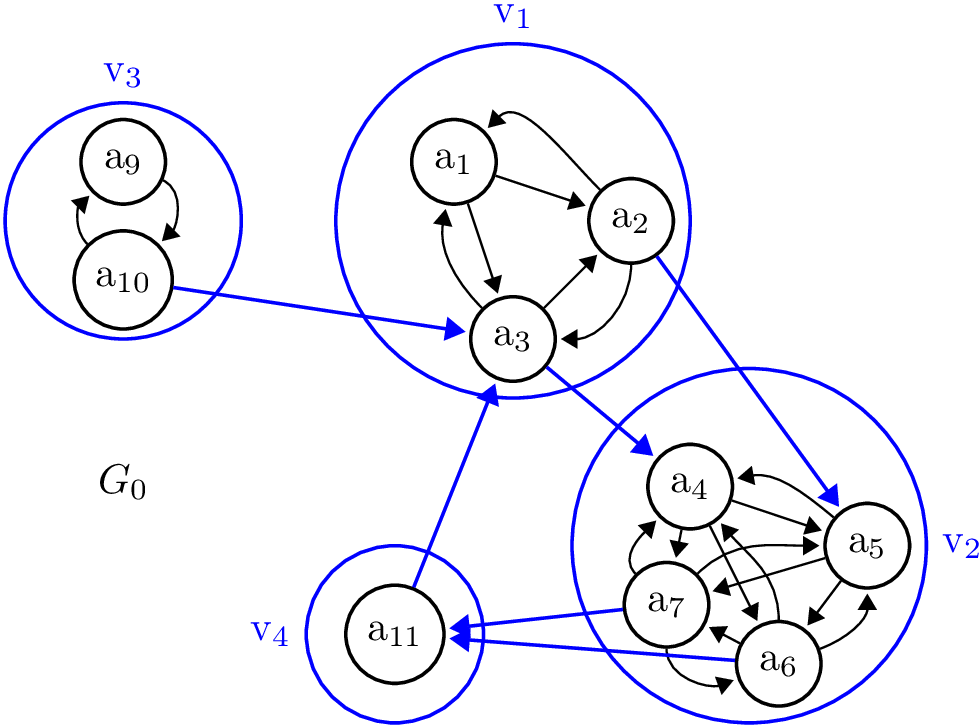
\includegraphics[scale=0.315]{Immagini/graph0.png}
    };

    \node[canvas is zy plane at x=5,draw,fill=white] at (0,0) {
        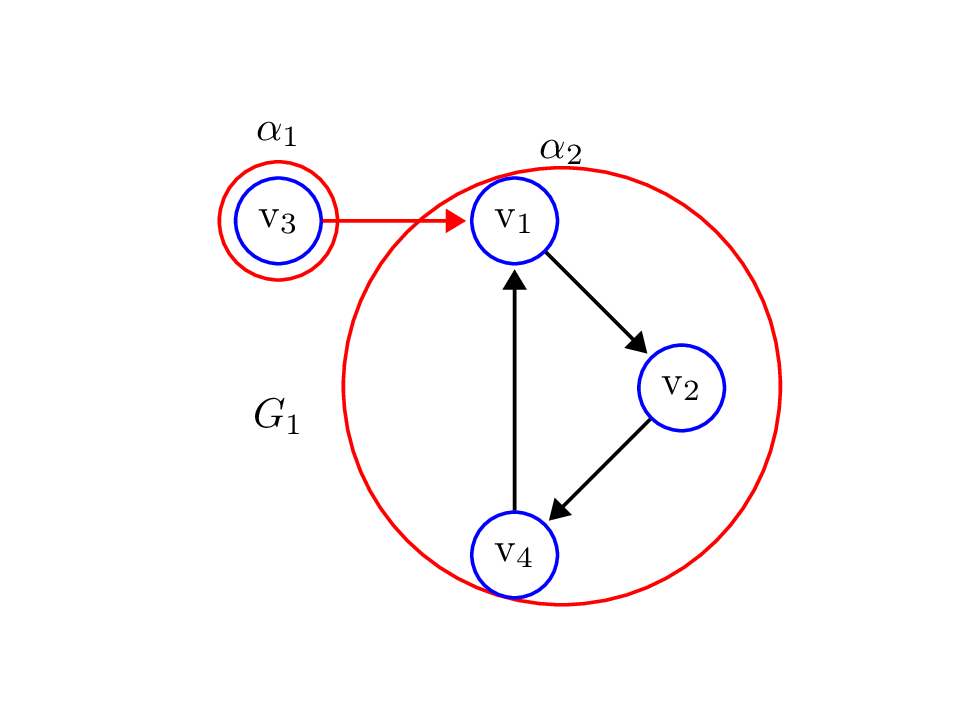
\includegraphics[scale=0.315]{Immagini/graph1.png}
    };

    \node[canvas is zy plane at x=10,draw,fill=white] at (0,0) {
        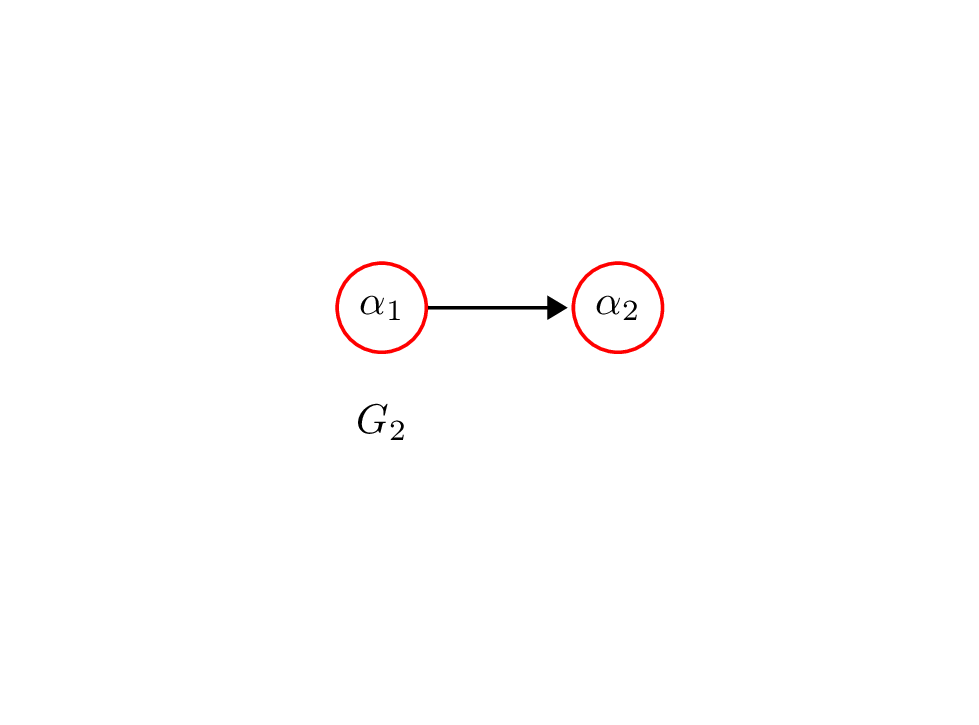
\includegraphics[scale=0.315]{Immagini/graph2.png}
    };
\end{tikzpicture}
    \caption{Esempio di grafo multilivello}
    \label{fig:multi-level-graph-example}
\end{figure}

\newpage

\nlparagraph{Algoritmo di trasformazione naturale}\label{subsec:algoritmo-di-trasformazione-naturale}

La generica procedura algoritmica per realizzare la trasformazione naturale di un grafo standard $H = (W, F)$
preso in input in un grafo decontraibile $G = (V, E, dec_V, dec_E)$, può essere definita considerando la creazione di
supernodi e superarchi, costruendo implicitamente la funzione biiettiva $f_V: W \rightarrow V$ che realizza
l'isomorfismo tra i nodi di $H$ e i supernodi di $G$.

\begin{algorithm}[H] \floatname{algorithm}{Algoritmo}
    \begin{algorithmic}[1]
        \caption{NATURAL-TRANSFORMATION($H$)}\label{alg:natural-transformation}
        \State Sia $G = (V, E)$ un nuovo grafo decontraibile, con $V = \emptyset$ e $E = \emptyset$
        \For{$x \in W$}
            \State Sia $v$ un nuovo supernodo
            \State $v.dec \coloneqq (\emptyset, \emptyset)$
            \State $V \coloneqq V \cup \{v\}$
        \EndFor
        \For{$(x,y) \in F$}
            \State Sia $e$ un nuovo superarco
            \State $e.dec \coloneqq \emptyset$
            \State $E \coloneqq E \cup \{e\}$
        \EndFor
        \State \Return $G$
    \end{algorithmic}
\end{algorithm}

Tramite l'ausilio di strutture dati con tempi di ricerca costanti, come insiemi di hash, la complessit\`a delle
operazioni all'interno dei due cicli \`e $O(1)$,
e, di conseguenza, la complessit\`a dell'algoritmo \`e dettata dal numero di nodi e archi del grafo in input $H$,
ovvero $\mathbf{\Theta(|W| + |F|)}$.